\documentclass[fontset=none,zihao=-4]{ctexart}
\setCJKmainfont{SimSun}[BoldFont=SimHei,ItalicFont=Adobe KaiTi Std]
\setCJKmonofont{FangSong}[BoldFont=SimHei,ItalicFont=Adobe KaiTi Std]
\newCJKfontfamily\kaishu{Adobe KaiTi Std}
\newCJKfontfamily\boldsong{Noto Serif CJK SC Bold}
\ctexset{section/format=\zihao{3}\bfseries\centering,paragraph/runin=false,paragraph/afterskip=1pt,bibname={参考文献}}
\linespread{1.15}
\usepackage{fontspec}
\usepackage{hyperref}
\usepackage{newpxtext}
\usepackage[vvarbb]{newpxmath}
\usepackage{bm}
\renewcommand\mathbf\bm
\defaultfontfeatures{}
\usepackage{graphicx}
\usepackage{physics}
\renewcommand\div\divisionsymbol
\usepackage{tabularray}
\UseTblrLibrary{amsmath}
\usepackage{tikz}
\usetikzlibrary{arrows.meta}
\usetikzlibrary{datavisualization.formats.functions}
\usepackage{geometry}
\geometry{top=3cm,bottom=3cm,left=2.5cm,right=2.5cm}
\usepackage[backend=biber,sorting=none]{biblatex}
\addbibresource{reference.bib}
\defbibheading{}

\begin{document}

\title{\boldsong\Large 宇宙线成像算法的研究}
\author{\zihao{4} 北京大学物理学院\ \ 2019级\ \ 张植竣}
\date{2022年10月24日}

\maketitle

\paragraph*{摘要}

自从宇宙射线被发现之后，宇宙射线相关领域的研究就成为了物理学中的热点问题。得益于宇宙射线具有的通量稳定、天然易获取、易探测、对人体和被探测物质无副作用等特点，利用宇宙射线对未知物体进行鉴别和成像是一个很有前景的研究领域。因为到达地面的宇宙射线中主要成分为μ子，所以宇宙射线成像核心问题就是利用μ子通过物质散射角和能量变化来对物质进行重构。大面积的宇宙射线成像系统的实现除了需要足够精度的探测器外，最重要的是成像算法。本文着重介绍了PoCA算法以及比例算法的原理，接着对算法进行实验，验证了这两种算法的成像效果。之后尝试考虑散射角的影响，对PoCA算法加以改进。

\clearpage\section{绪论}

\subsection{宇宙线简介}

1912年，奥地利物理学家Hess利用热气球在5300米高空的电离实验，观测到在1000米以下，大气电离率逐渐下降，但随后出现明显上升。这首次给出了可能存在来自宇宙的高穿透性辐射的证据。后来科学家使用宇宙射线来泛指来自外太空的高能粒子及其次级粒子。自从宇宙射线被发现之后，与之相关领域的研究就成为了物理学中的热点问题。

宇宙射线分为初级宇宙射线和次级宇宙射线，来自外太空的初级宇宙射线，其主要成分为约89\%的质子，约10\%的α粒子和少量的重元素核，其余1\%中绝大部分是电子，只有极小的一部分是γ射线、超高能中微子等。初级宇宙射线进入大气层，与大气中的分子多次碰撞，发生大量的高能核反应，产生许多游离的粒子和电磁辐射。这个过程被称为“大气簇射（air shower）”。这些粒子在大气中不稳定，很快就会衰变为μ子、电子、γ射线等，形成次级宇宙射线。到达海平面的的宇宙射线中主要成分是是μ子，其通量占总通量的75\%。剩余的主要是正负电子以及光子。宇宙射线中的μ子，平均能量在$3 \sim 4\,\mathrm{GeV}$之间。μ子的流强约为每分钟每平方厘米一个，速度接近光速。

宇宙线的来源多种多样。太阳耀斑产生相对低能量的宇宙射线，以高能质子为主，能够穿透地球磁场。很大一部分初级宇宙射线来自于银河系内部的超新星遗迹。除此之外，可能会辐射宇宙射线的备选体包括但不限于白矮星、中子星（磁星）、X射线双星等等。我们观测得到的河外宇宙射线主要在高能范围内，来源有γ射线暴、活动星系核、星系团等。由于绝大部分宇宙线粒子都是带电粒子，会在宇宙磁场中偏转，对宇宙线来源的寻找带来了极大挑战，期待更先进的探测设备带来更多的数据。

宇宙线的能量跨越了11个数量级，约$10^9\,\mathrm{eV} \sim 10^{20}\,\mathrm{eV}$。Fermi在1949年提出“Fermi加速机制”解释了宇宙线粒子的高能量：粒子与星际介质云的磁场碰撞而获得加速。宇宙线流量$I$与能量$E$的关系在如此大的范围内几乎没有偏离$I \propto E^{-2.7}$的常数幂律分布。Greisen-Zatsepin-Kuzmin极限（GZK极限）是高能质子从其他星系穿过星系际介质到达我们星系的能量的理论上限，约为$5 \times 10^{19}\,\mathrm{eV}$，原因是会和宇宙微波背景辐射相互作用。

\subsection{宇宙线的探测}

目前使用的几种地面检测宇宙射线的方法，可以分为两大类：各种类型的粒子探测器探测大气簇射中的次级宇宙射线粒子以及探测大气中宇宙线与分子碰撞发出的电磁辐射。

粒子探测器主要有气体探测器与固体探测器两种。气体探测器结构为两块相互平行的金属极板，其间填充适量的工作气体，极板之间加上一定电压，这样便在中间的气隙中形成匀强电场。当有粒子穿过气隙时，电离产生的电子离子对在电场的作用下加速促使更多的原子电离。这种电离不断增值的过程叫做电子雪崩过程，使得极板读出条上感应出电流，电流从延迟块两端输出，通过这两路输出和时间路的复合及其他操作得到带电粒子的位置。固体探测器的主要结构是闪烁体和光电倍增管。入射辐射引起闪烁体中原子（或离子、分子）的电离激发，之后受激粒子退激发，放出波长接近于可见光的闪烁光子。闪烁光子通过光导射入光电倍增管的光阴极并打出光电子，光电子受电极之间强电场的作用加速运动并轰击下一电极，打出更多光电子，由此实现光电子的倍增，直到最终到达阳极并在输出回路中产生信号。

探测电离辐射主要使用Cherenkov辐射探测器。Cherenkov辐射是介质中运动的电荷速度超过该介质中光的相速度时发出的一种以短波长为主的电磁辐射，其特征是蓝色辉光。一个常见的类比是超音速飞机的音爆：飞机产生的声波以比飞机慢的声速行进，不能从飞机向前传播，反而形成锥形的冲击锋。类似地，Cherenkov辐射可以说是带电粒子在穿过介质时产生的光“冲击波”。通过建设巨大的水池和光电倍增管阵列，或者空气Cherenkov望远镜，可以探测到大量高能粒子产生的Cherenkov辐射。

我国在宇宙线探测方面走在世界前列。2021年，在海拔$4410\,\mathrm{m}$的四川省稻城县海子山建成高海拔宇宙线观测站（LHAASO），由地面簇射粒子阵列、水Cherenkov探测器阵列和广角Cherenkov望远镜阵列组成。在还不算长的观测时间中，已经发现了目前探测到的能量最高的γ光子，达到$1.4\,\mathrm{PeV}$，发现大量超高能宇宙加速器，精确测量蟹状星云亮度等，开启了 “超高能γ天文学”时代。

\subsection{μ子成像技术及其应用}

因为宇宙射线中μ子通量稳定、穿透能力强、易获取、对人体无害，而且μ子带电，可以直接被闪烁体探测器、气体探测器等简单高效的器件探测。所以宇宙射线成像主要是利用μ子进行成像。

μ子成像技术主要分为两类，一类是利用μ子通过物质时被吸收而能量衰减的规律还原μ子透过的物体的性质，另一类技术是利用物质对μ子的散射特性进行成像。物体对μ子的小角度散射基本服从均值为0的Gauss分布，大角度表现为Rutherford散射，且原子核越重，散射强度越大。由文献\cite{schultz2003cosmic}可以知道即使对于重核，μ子的散射角也很小：$3\,\mathrm{GeV}$能量的μ子穿透$10\,\mathrm{cm}$的铀层，散射角的方均根值是$1.6^\circ$。这对使用散射谱进行成像对探测器的精度和还原算法的有效性提出了很高的要求。美国Los Alamos实验室于2003年提出PoCA算法\cite{schultz2004image}，2007年提出MLSD算法\cite{schultz2007statistical}，这两个算法是在宇宙射线成像算法方面具有突破性进展的一步。

μ子的强穿透能力使它可以穿透很厚的屏蔽层从而用于对重元素材料的检测。例如在1955年，George利用μ子注量在地下的衰减测量了岩层的厚度。后来Alcarez等人将该方法应用于大的建筑物考古成像及地质结构的测量，例如胡夫大金字塔。近年来μ子成像技术得到了关注和研究，即利用μ子穿过原子量不同的物质时具有不同的散射角的原理，对大型物质进行辐射成像。这种新型的检测方法应用于核安全领域，能够有效探测到封装良好的核材料，如$^{235}\mathrm{U}$、$^{239}\mathrm{Pu}$等。

\clearpage\section{宇宙射线成像算法}

\subsection{基本原理}

本文所指的宇宙射线成像系统都是μ子成像系统。图1就是成像系统结构的简单示意图。通常将两组对称的μ子探测器放在成像区域的两侧，每组至少两块能够测量粒子在板所在平面上二维位置的探测板。通过这两组探测器的复合，可以测量μ子的入射矢量和出射矢量及对应的方位角。通过额外的μ子接收器可以得到μ子的动量。图1中灰色带箭头的轨迹代表经过空气散射的μ子，黑色带箭头的轨迹代表经过重核物质散射的μ子。由于后者的散射角明显大于前者，于是我们可以通过在大量粒子经过成像系统后统计学上性质还原出成像区域的散射特征。

\begin{figure}[ht]
    \centering
    \includegraphics[width=0.75\linewidth]{muon.png}
    \caption{\kaishu μ子成像系统示意图}
\end{figure}

考虑μ子穿过一定厚度的单层均匀介质。定义μ子的入射和出射矢量之间的夹角为总散射角$\theta$，对常见材料来说，可以认为$\theta$服从平均值为0的Gauss分布：
\[
    f(\theta) = \frac{1}{\sigma_\theta\sqrt{2\pi}} \exp(-\frac{\theta^2}{2\sigma_\theta^2})
\]
文献\cite{hagiwara2002review}中指出$\sigma_\theta$满足：
\[
    \sigma_\theta = \frac{E_0}{p\beta c} \sqrt{\frac{L}{L_{\mathrm{rad}}}} \left[1 + 0.0038\ln\frac{L}{L_{\mathrm{rad}}}\right] \approx \frac{E_0}{p\beta c} \sqrt{\frac{L}{L_{\mathrm{rad}}}}
\]
其中$E_0 = 13.6\,\mathrm{MeV}$，$p$和$\beta$为μ子的动量和速度，$L$是μ子经过的距离（近似于散射物质的厚度）。$L_{\mathrm{rad}}$是材料的散射长度，定义为高能电子通过轫致辐射能量衰减到原来的$\mathrm{e}^{-1}$经过的平均长度，与物质的原子序数$Z$和密度$\rho$有关，是物质的固有属性。

定义散射强度：
\[
    \lambda = \left(\frac{E_0}{p_0\beta c}\right)^2 \frac{1}{L_{\mathrm{rad}}} = \left(\frac{p}{p_0}\right)^2 \frac{\sigma_\theta^2}{L}
\]
其中$p_0 = 3\,\mathrm{GeV}/c$。统计上，若总共有$N$个入射μ子，根据标准差的定义有：
\[
    \lambda = \frac{1}{N} \sum_{i=1}^N \left(\frac{p_i}{p_0}\right)^2 \frac{\theta_{xi}^2 + \theta_{yi}^2}{2L_i}
\]
表1列举了几种常见金属的散射长度$L_{\mathrm{rad}}$和散射强度$\lambda$。一般来讲，原子序数$Z$越高，物质密度$\rho$越大，则$L_{\mathrm{rad}}$越小，$\lambda$越大。

\begin{table}[ht]
    \centering
    \begin{tabular}{|c|c c c c|}
        \hline
        材料 & W & Pb & Fe & Al \\
        \hline
        $Z$ & 74 & 82 & 26 & 13 \\
        \hline
        $L_{\mathrm{rad}} / \mathrm{cm}$ & 0.35 & 0.56 & 1.76 & 8.90 \\
        \hline
        $\lambda / (\mathrm{rad^2 \cdot m^{-1})}$ & 0.00587 & 0.00367 & 0.00117 & 0.00023 \\
        \hline
    \end{tabular}
    \caption{\kaishu 几种常见金属的散射长度$L_{\mathrm{rad}}$和散射强度$\lambda$}
\end{table}

\subsection{PoCA算法}

PoCA（Point of Closest Approach）算法是最常见的宇宙射线成像算法之一，具有速度快，实现简单等特点，最早由Schultz等人在文献\cite{schultz2004image}中提出。PoCA算法的核心思想是对μ子多次Coulomb散射过程近似为一次等效散射。这个散射点我们称它为PoCA点。在实际的成像系统中，μ子发生的是多次散射，我们取μ子入射矢量延长线与出射矢量延长线的公垂线段的中点为PoCA点。

PoCA算法的基本步骤如下：
\begin{itemize}
    \item[\textcircled{1}] 将成像区域均匀分割成若干小体积元，对成像区域的某一个体积元$j$，入射的μ子数$N_j$初始化为0，$\lambda_j$也为0。

    \item[\textcircled{2}] 对第$i$个μ子计算其PoCA点。假设入射点和出射点坐标分别为$\mathbf{P}_i$和$\mathbf{P}_o$，入射矢量和出射矢量分别为$\mathbf{v}_i$和$\mathbf{v}_o$，那么计算PoCA点的步骤为：
    \begin{itemize}
        \item[\bullet] 入射矢量和出射矢量归一化为单位矢量$\mathbf{n}_i$和$\mathbf{n}_o$。
        \item[\bullet] 公垂线段的方向矢量（单位矢量）为$\mathbf{n} = \dfrac{\mathbf{n}_i \times \mathbf{n}_o}{\abs{\mathbf{n}_i \times \mathbf{n}_o}}$，长度为$d = (\mathbf{P}_o - \mathbf{P}_i) \cdot \mathbf{n}$。

        \item[\bullet] 将$\mathbf{P}_i$沿$\mathbf{n}$平移$d$长度，得到点$\mathbf{P}_1 = \mathbf{P}_i + d\mathbf{n}$。

        \item[\bullet] 将$\mathbf{P}_1$沿入射方向$\mathbf{n}_i$平移$l_1 = (\mathbf{P}_o - \mathbf{P}_1) \cdot \mathbf{n}_i$长度，得到点$\mathbf{P}_2 = \mathbf{P}_1 + l_1\mathbf{n}_i$。

        \item[\bullet] 将$\mathbf{P}_2$沿出射反方向$-\mathbf{n}_o$方向平移$l_2 = \dfrac{\abs{\mathbf{P}_o - \mathbf{P}_2}^2}{(\mathbf{P}_o - \mathbf{P}_2) \cdot \mathbf{n}_o}$长度，得到点$\mathbf{P}_3 = \mathbf{P}_o - l_2\mathbf{n}_o$。这个点就是公垂线段在出射轨迹延长线上的交点。

        \item[\bullet] 将$\mathbf{P}_3$沿$-\mathbf{n}$平移$\dfrac{d}{2}$长度得到PoCA点$\mathbf{M} = \mathbf{P}_3 - \dfrac{d}{2}\mathbf{n}$。
    \end{itemize}

    \item[\textcircled{3}] 以入射点、PoCA点和出射点所连的两段折线作为该μ子在物体中运动的近似轨迹。在PoCA点所在的体积元，计算：
    \[
        \lambda_{ij} = \left(\dfrac{p_i}{p_0}\right)^2 \dfrac{\theta_{xi}^2 + \theta_{yi}^2}{2L_i}
    \]

    \item[\textcircled{4}] 对轨迹经过的每一个体积元，$N_j = N_j + 1$，对于PoCA点所在的体积元，$\lambda_j = \lambda_j + \lambda_{ij}$。

    \item[\textcircled{4}] 计算完所有μ子的入射事件后，对所有体积元执行：$\lambda_j = \dfrac{\lambda_j}{N_j}$
\end{itemize}

\subsection{比例算法}

文群刚等在文献\cite{liu2020study}中提出了比例算法。原理是将$\sigma_\theta$分成两部分：与材料有关的常数$H$和与材料无关的常数$A$，方法如下：
\[
    \sigma_\theta = \frac{H}{p},\quad H = \frac{E_0}{\beta c} \sqrt{\frac{L}{L_{\mathrm{rad}}}} \left[1 + 0.0038\ln\frac{L}{L_{\mathrm{rad}}}\right]
\]
由于$(1-\beta) \ll 1$，$H$可以看成是只与材料有关的常数。

将散射事件按照μ子的动量分为$n$组，每组有$k_i$个事件，且$\expval{\theta}_i = 0$，则有：
\[
    \sigma_i = \frac{1}{k_i}\sum_{j=1}^{k_i} \theta_{ij}^2 = \frac{H^2}{p_i^2}
\]
再对每一组求和：
\[
    \sigma_\theta^2 = \frac{1}{N}\sum_{i=1}^N \theta_i^2 = \sum_{i=1}^n \frac{k_i}{N}\frac{H^2}{p_i^2}
\]
如果实验数据足够，μ子的动量分布应该满足自然界的稳定分布，于是可以令常数：
\[
    A = \sum_{i=1}^n \frac{k_i}{N}\frac{1}{p_i^2}
\]
且有：$\lim\limits_{n \to \infty} A = \expval{\dfrac{1}{p^2}}$。最后就有：
\[
    \sigma_\theta^2 = AH^2
\]
可以看出，μ子的动量误差对最终结果的影响可以忽略不计。实际上只需要处理位置数据而不需要动量数据。

由于散射角是一个Gauss分布，标准差$\sigma_\theta$随散射体的$Z$增大而增大。计算一定角度$\theta_0$内散射的事件占总事件数之比：
\[
    R = \frac{A_{\theta_0}}{A_0} = \frac{1}{\sigma_\theta\sqrt{2\pi}} \int_{-\theta_0}^{\theta_0} \exp(-\frac{\theta^2}{2\sigma_\theta^2}) \dd{\theta}
\]
比例$R$越低，散射体的$Z$也就越大。该算法的优点是几乎不利用散射角数据本身，提取有效数据，μ子动量的误差对散射角标准差影响较小；其局限性则是不能判断散射体的位置（仍然依赖PoCA算法）。

\clearpage
\section{宇宙射线成像模拟}

\subsection{RPC阻性板气体探测器介绍}

经典的平行板型气体探测器使用金属作为电极，这带来了一个问题：当一个粒子入射探测器发生雪崩后，极板之间的电压会因为放电而在短时间内降低，气隙中的电场减弱，脱离工作状态，此时若有其他粒子入射，探测器将无法做出有效的响应。金属是导体，所以电场强度的降低不只发生在粒子入射的区域，而是遍及整个气隙，这严重限制了探测器的计数率本领。为了在高计数率环境下工作，用阻性板电极替代金属电极并进行改良，衍生出的平行板型气体探测器就是阻性板室（Resistive Plate Counter，RPC）。为了使电压均匀地分配到各处，阻性板的外表面常常喷涂石墨层来施加电压。阻性板探测器因为其结构简单、工作稳定、制作成本低廉的特点在核物理核高能实验中被广泛应用。

\subsection{模拟实验}

这部分实验建立在使用Geant4模拟的虚拟实验平台上。如图2所示，四块标有线框的板是RPC探测器的四块玻璃板。探测器有效面积为$200\,\mathrm{mm} \times 200\,\mathrm{mm}$，四块玻璃板的间距均为$300\,\mathrm{mm}$。探测器中央有一个边长为$60\,\mathrm{mm}$的钨立方体，以立方体中心的位置为坐标原点，竖直方向为$z$方向。

\begin{figure}[ht]
    \centering
    \includegraphics[width=0.35\linewidth]{RPC.png}
    \caption{\kaishu RPC探测器示意图}
\end{figure}

\subsection{PoCA算法改进}

通过数学计算，可以将PoCA算法的实现改为三步：
\begin{itemize}
    \item 公垂线段的方向矢量（单位矢量）为$\mathbf{n} = \dfrac{\mathbf{v}_i \times \mathbf{v}_o}{\abs{\mathbf{v}_i \times \mathbf{v}_o}}$，长度为$d = (\mathbf{P}_o - \mathbf{P}_i) \cdot \mathbf{n}$。

    \item 将$\mathbf{P}_i$沿$\mathbf{n}$方向平移$t_i \mathbf{v}_i$长度，得到点$\mathbf{P}'_1 = \mathbf{P}_i + t_i \mathbf{v}_i$。其中$t_i$由以下方程决定：
    \[
        \mathbf{P}_i + t_i \mathbf{v}_i + d \mathbf{n} = \mathbf{P}_o - t_o \mathbf{v}_o
    \]
    通过解三个分量方程（实际上只需要两个），可以得到：
    \[
        t_i = \frac{(P_{ox} - P_{ix} - dn_x)v_{oy} - (P_{oy} - P_{iy} - dn_y)v_{ox}}{v_{ix}v_{oy} - v_{iy}v_{ox}}
    \]
    \[
        t_i = \frac{(P_{ox} - P_{ix} - dn_x)v_{oy} - (P_{oy} - P_{iy} - dn_y)v_{ox}}{v_{ix}v_{oy} - v_{iy}v_{ox}}
    \]

    \item 将$\mathbf{P}'_1$沿$\mathbf{n}$平移$\dfrac{d}{2}$长度得到PoCA点$\mathbf{M} = \mathbf{P}'_1 + \dfrac{d}{2}\mathbf{n} = \mathbf{P}_i + t_i \mathbf{v}_i + \dfrac{d}{2}\mathbf{n}$。
\end{itemize}

使用简化后的PoCA算法，计算PoCA点的时间减少到了原来的40\%（从$0.025\,\mathrm{s}$下降到$0.01\,\mathrm{s}$），在1000000个粒子入射事件中得到的结果如图4所示。其中空间分辨率（单元格边长）为$3\,\mathrm{mm}$，纵坐标$\lambda/\lambda_0$为约化后的值。$\lambda_0 = 0.00587\,\mathrm{rad^2/m}$。

从图中可以看出，PoCA算法在$x$方向和$y$方向还原出的物体边缘较为清晰准确，但是$z$方向偏离较大，峰值大约在$22.5\,\mathrm{mm}$，相比正确值$0\,\mathrm{mm}$偏上，部分单元格的$\lambda$过高。

从原理上，$z$方向成像误差较大的原因是使用一次散射近似多次散射而不考虑整个散射过程，而且宇宙射线中μ子的入射角一般接近竖直方向（$z$方向）。如图，散射角（入射角）的较小误差$\Delta\theta$就会导致PoCA点的位置从$\mathbf{M}$变化到$\mathbf{M}'$，在$z$方向表现为巨大误差。

\begin{figure}[ht]
    \centering
    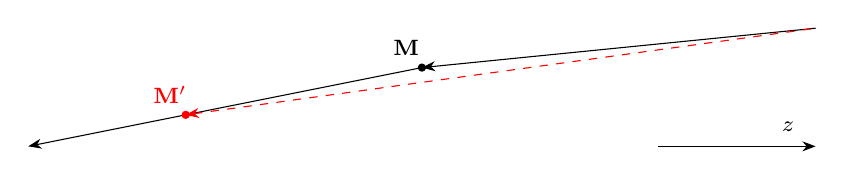
\begin{tikzpicture}[>=Stealth]
        \draw [->] (3,0) -- (5,0);
        \draw (4.65,0.25) node {\footnotesize$z$};
        \draw [<-] (-5,0) -- (0,1);
        \draw [<-] (0,1) -- (5,1.5);
        \draw [<-,color=red,dashed] (-3,0.4) -- (5,1.5);
        \fill (0,1) circle [radius=1.5pt];
        \fill [red] (-3,0.4) circle [radius=1.5pt];
        \draw (-0.2,1.25) node {\footnotesize$\mathbf{M}$};
        \draw (-3.2,0.65) [red] node {\footnotesize$\mathbf{M}'$};
    \end{tikzpicture}
    \caption{\kaishu PoCA算法$z$方向误差的示意图}
\end{figure}

下面是其中一次实验中不同大小散射角的统计结果：

\begin{table}[ht]
    \centering
    \begin{tabular}{|c|c c c c c c c|}
        \hline
        散射角$\theta$ & $[0^\circ,+\infty)$ & $[0^\circ,1^\circ)$ & $[1^\circ,2^\circ)$ & $[2^\circ,3^\circ)$ & $[3^\circ,4^\circ)$ & $[4^\circ,5^\circ)$ & $[5^\circ,+\infty)$ \\
        \hline
        事件数$N$ & 44547 & 23487 & 8566 & 4099 & 2400 & 1559 & 4436 \\
        \hline
    \end{tabular}
    \caption{\kaishu 不同大小散射角的事件数}
\end{table}

可见，绝大多数散射角都在$5^\circ$以下，其中大部分小于$1^\circ$，说明大部分事件都在$z$方向有较大的不确定度。但是散射角过大，则可能使得PoCA点处于探测器外而不符合物理事实。一种简单直接的解决方法是舍去小角度和过大角度的数据，缺点是大量的数据无法使用，事件利用率较低。

另一方面，PoCA点的位置是数学上相对确定的，也就是说，如果计算出PoCA点的$z$坐标为$z_1$，真实坐标为$z_2$，我们无法从$z_1$中估计$z_2 - z_1$以逼近$z_2$。所以，获得更好的分辨率必须从$\lambda$的计算入手。

考虑对散射角为$\theta$（以弧度为单位）的粒子事件进行如下操作：
\begin{itemize}
    \item 设置标准差$\sigma = K\theta$，这里取$K = 100$。

    \item 对于正态分布$N(0,\sigma)$，在$[-n,n]$以内的分布概率是$\erf\left(\dfrac{n}{\sigma\sqrt{2}}\right)$，于是有：
    \[
        \delta_1 = \erf\left(\frac{1}{\sigma\sqrt{2}}\right),\quad
        \delta_2 = \frac{1}{2}\left(\erf\left(\frac{2}{\sigma\sqrt{2}}\right) - \delta_1\right),\quad
        \delta_3 = \frac{1}{2} - \frac{1}{2}\delta_1 - \delta_2
    \]

    \item 在PoCA散射点$\mathbf{M}(x,y,z)$处，$\lambda_{ij} = \delta_1\Delta\lambda$，在$(x,y,z+1)$和$(x,y,z-1)$的位置，$\lambda_{ij} = \delta_2\Delta\lambda$，在$(x,y,z+2)$和$(x,y,z-2)$的位置，$\lambda_{ij} = \delta_3\Delta\lambda$。
\end{itemize}

得到的结果如图5、图6、图7所示。

可以看出$z$方向$\lambda$的峰值改进到$13.5\,\mathrm{mm}$处，且图像更加平滑，边缘更清晰，部分单元格的$\lambda$过高的问题也得到了明显改善。通过改变$K$的值可以得到不同的结果，但$K>100$后输出结果对$K$值不敏感。

\subsection{比例算法}

在研究组2014年的测试中，使用有效边长为$203\,\mathrm{mm} \times 203\,\mathrm{mm}$的RPC探测器对边长为$30\,\mathrm{mm}$的正方体木块、铁块和铅块做了成像实验。这里运用比例算法（此处计算PoCA点时舍弃了所有散射角小于$3.6^\circ$的事件）得到的结果如图8、图9、图10所示。

如图，比例算法在识别物质的$Z$值分布时具有边缘清晰，对比度好的特点。其中一个原因是使用了随机重构参考点的方法：以重构点为中心取一个立方体区域，在这个区域内计算$\sigma_\theta$和$R$。通过随机重构点可以大限度地利用实验数据点，从而实现少数据量的成像。缺点是运行速度慢（运行一次需要约$40\,\mathrm{s}$，相比之下PoCA算法处理相同大小的数据只需要约$1\,\mathrm{s}$），且舍弃了大量的PoCA点数据。

\clearpage

\begin{figure}[!ht]
    \centering
    \includegraphics[width=0.4\linewidth]{poca_x.png}
    \quad
    \includegraphics[width=0.4\linewidth]{poca_z.png}
    \caption{\kaishu PoCA算法$x$方向（左）和$z$方向（右）的成像结果}
\end{figure}

\begin{figure}[!ht]
    \centering
    \includegraphics[width=0.75\linewidth]{poca_z_2.png}
    \caption{\kaishu 改进后PoCA算法$z$方向的成像结果}
\end{figure}

\clearpage

\begin{figure}[!ht]
    \centering
    \includegraphics[width=0.4\linewidth]{poca_z.png}
    \quad
    \includegraphics[width=0.4\linewidth]{poca_z_2.png}
    \caption{\kaishu 改进前（左）与改进后（右）PoCA算法$z$方向的成像结果对比}
\end{figure}

\begin{figure}[!ht]
    \centering
    \includegraphics[width=0.75\linewidth]{poca_3D.png}
    \caption{\kaishu 改进后PoCA算法的三维成像结果（紫端表示$\lambda$较小，黄端表示$\lambda$较大）}
\end{figure}

\clearpage

\begin{figure}[!ht]
    \centering
    \includegraphics[width=0.4\linewidth]{pbtofe.png}
    \quad
    \includegraphics[width=0.5\linewidth]{P_R_1.png}
    \caption{\kaishu 8个铅块与8个铁块}
\end{figure}

\begin{figure}[!ht]
    \centering
    \includegraphics[width=0.4\linewidth]{pbinfe.png}
    \quad
    \includegraphics[width=0.5\linewidth]{P_R_2.png}
    \caption{\kaishu 56个铁块包裹8个铅块}
\end{figure}

\begin{figure}[!ht]
    \centering
    \includegraphics[width=0.4\linewidth]{woodinfe.png}
    \quad
    \includegraphics[width=0.5\linewidth]{P_R_3.png}
    \caption{\kaishu 56个铁块包裹8个木块}
\end{figure}

{\kaishu 注：左侧是实验装置示意图。右侧是散射角标准差$\sigma_\theta$与比例$R$的图像，其中只选取了散射角在$3.6^\circ$和$20^\circ$之间的事件。上半部分是散射角分布，下半部分是计算出的比值$R$。注意$\sigma_\theta$随散射物质的$Z$增大而增大，而$R$随$Z$增大而减小。全部图像的颜色映射都是紫端表示数据较小，黄端表示数据较大。}

\clearpage\section{结论}

本文首先介绍了宇宙射线、μ子探测技术的历史背景及应用，接着着重介绍了PoCA算法以及比例算法的原理。我们使用Geant4的模拟数据和RPC的实测数据对两种算法进行实验，验证了这两种算法的成像效果。实验发现PoCA算法简单高效，在有效数据点数足够时能很好地重构原物体，但是$z$方向的成像质量比$x$方向和$y$方向的差。比例算法在识别物质的$Z$值分布时具有数据量较少时边缘清晰，对比度好的特点，缺点是运行速度慢，对PoCA点数据的利用率不高。最后考虑散射角的影响，在计算散射强度$\lambda$时引入$z$方向的不确定度，改进了PoCA算法，提高了其在$z$方向的成像质量。

\section*{\zihao{-4} 致谢}

首先要感谢的是指导教师李奇特老师，在研究中李老师对我进行了耐心细致的指导，给我提出了许多有建设性的建议，启发了我的研究思路。老师还给予我许多研究和实习的机会，例如参与了2021年7月在中科大举办的国内μ子成像技术与应用研讨会，采购研究组所需的服务器等。

其次是我们气体探测器小组的几位同学：赵月悦、边佳伟和刘承恩。他们的工作虽然与我不同，但是很有启发性，十分值得借鉴，在研究过程中也得到了他们的很多帮助。此外我们都参与组装了大面积闪烁体中子墙探测器。

最后是在我之前研究成像算法的两位学长叶亚杰和卜逸舟。我的算法的原始版本就是他们提供的。如果没有他们的工作，那么我的研究就好比空中楼阁一般根本无法开展,因此他们的贡献是决定性的。

\paragraph*{参考文献}

\printbibliography[heading=none]

\paragraph*{作者简介}

张植竣，男，2001年8月出生于广州，2019年从华南师范大学附属中学考入北京大学物理学院。该生在思想道德方面表现良好，尊重师长，与同学相处融洽。申请人本科数学物理课程和专业课程均取得了优秀的成绩，有良好的数理基础。在几门课的课堂上表现活跃，积极思考，求知欲强，勇于提问，也取得了很好的成绩，给老师留下了很深的印象。能够对学到的知识思考和质疑，从而达到掌握运用，是很好的学习习惯，也是将来从事科研的良好基础。在课后，申请人也经常和同学积极开展讨论，易于沟通交流，有乐观的心态和端正的学习态度。

\paragraph*{感悟与寄语}

通过本科生科研，我有幸参与到了科研工作当中。我的学习能力和研究能力得到了有效提高。面对从未接触过的C++语言、CERN ROOT数据处理工具和Geant4模拟，我努力学习，掌握了许多编程和数据处理的技巧，对研究组的代码进行了许多改进。参加全国性的研讨会扩展了我的学术视野，让我对该领域的发展有了更清晰的认知。参与组装种子探测器和购买实验室服务器让我认识到物理研究也需要脚踏实地，从最基础的工作开始做起。

\paragraph*{指导教师简介}

李奇特，男，博士，高级工程师。1985年11月出生于海南澄迈。2012年博士毕业于北京大学粒子物理与核物理专业。2012年起在北京大学技术物理系、核物理与核技术国家重点实验室（北京大学）工作，主管北京大学物理学院亚原子粒子探测实验室，主要工作方向为实验核物理、辐射探测器研发。主持或参加了国家自然科学基金重大科研仪器研制项目、面上项目、青年科学基金项目以及国家重点研发计划课题。完成了AT-TPC、RPC探测器和宇宙射线成像系统的研发，参与建设了国内首台共线激光核谱仪，推进了多个在束核物理实验研究。曾获国家重点实验室科研成果奖、工程技术奖。任核仪器行业协会理事，任JINST和NST等学术期刊审稿人。

\end{document}